%% !TeX root = report.tex

\paragraph{Zbiór large}

Pierwszym przeprowadzonym testem był test wszystkich wersji algorytmu dla zbioru {\em large}. Rozmiar bloku BWT ustawiony został na wartość równą 4 MB, czyli nieco mniejszą niż rozmiar największego pliku.

\begin{figure}[phtb]
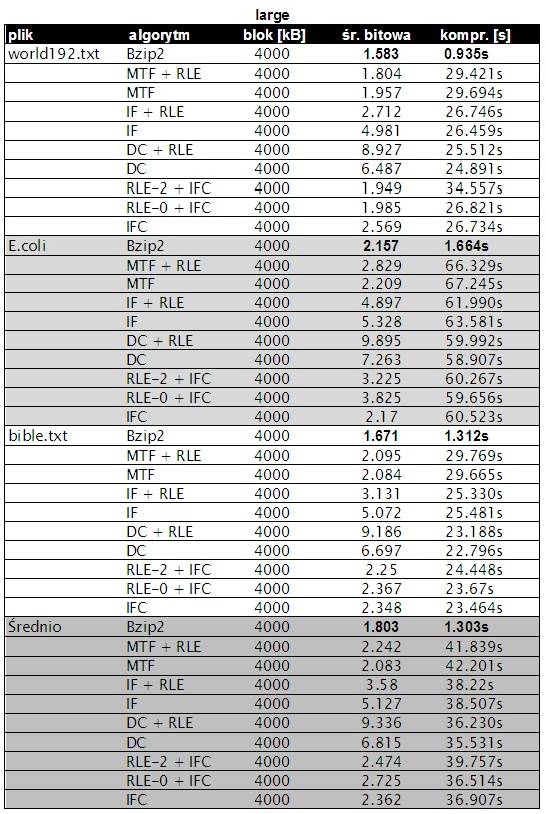
\includegraphics[scale=1.0]{\PICSDIR/tab_large_wszystkie.jpg}
\caption{\label{fig:tab_large_wszystkie}Wyniki testu dla zbioru large}
\end{figure}

Dla tych plików najlepszym okazał się referencyjny algorytm Bzip2, jednak pod względem wartości średniej bitowej niewiele gorszy okazał się algorytm MTF. Różnica wynosi jedynie 15 proc. Następne miejsce zajął algorytm MTF+RLE, a kolejne algorytmy wykorzystujące IFC. Dużo gorzej wypadły metody IF i DC.
 
Niestety pod względem czasu trwania kompresji nasz algorytm znacznie odbiegał od Bzip2. Najdłużej działała metoda, która uzyskała najlepszy wynik pod względem wartości średniej bitowej (MTF) i czas ten był aż 32 razy dłuższy od referencyjnego Bzip2.

\paragraph{Badanie wpływu rozmiaru bloku BWT}

\begin{figure}[phtb]
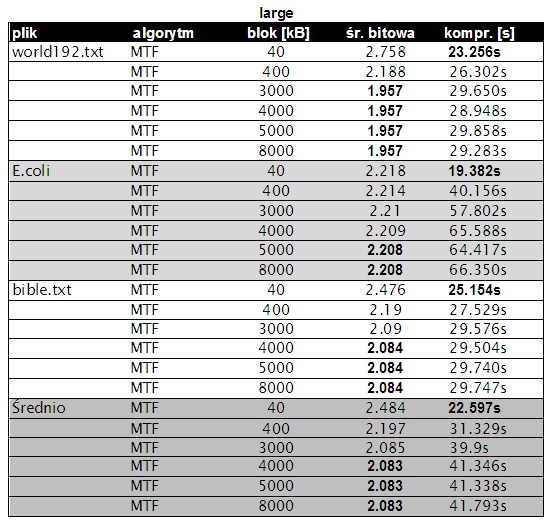
\includegraphics[scale=1.0]{\PICSDIR/tab_large_badanieBlokSize.jpg}
\caption{\label{fig:tab_large_badanieBlokSize}Wyniki testu parametru rozmiaru bloku BWT dla zbioru large}
\end{figure}

Algorytm, który uzyskał najlepszą średnią bitową w poprzednim teście posłużył do wykonania testu wpływu wartości parametru rozmiaru bloku BWT na jakość kompresji. Zgodnie z przewidywaniami, im większa wartość bloku tym algorytm BWT lepiej radzi sobie z kompresją, ale wzrasta długość trwania kompresji. Ograniczeniem jest długość samego pliku poddawanego poszczególnym operacjom. W dalszych testach wartość tego parametru pozostała na poziomie 4 MB, gdyż tylko rozmiar jednego z testowanych plików przekracza tą wartość, a dalszy wzrost tego parametru poprawia średnią bitową dla tego pliku o mniej niż jeden promil.

\paragraph{Zbiór canterbry}

\begin{figure}[phtb]
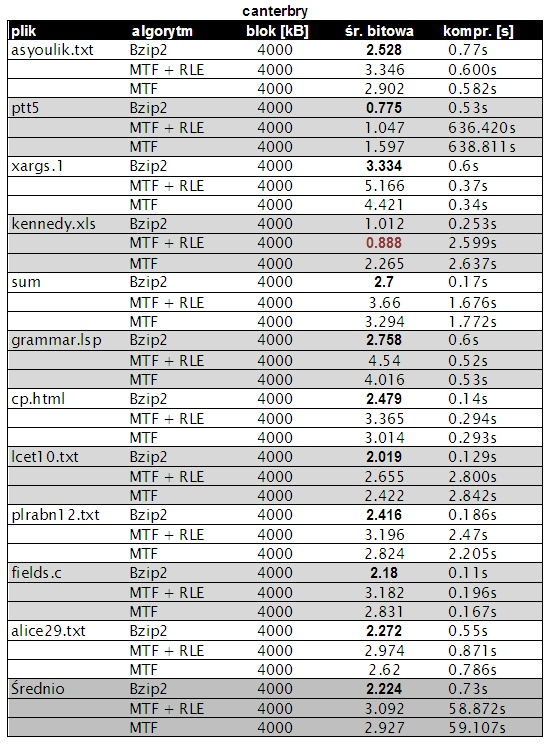
\includegraphics[scale=1.0]{\PICSDIR/tab_canterbry_lepszyNizBzip2.jpg}
\caption{\label{fig:tab_canterbry_lepszyNizBzip2.jpg}Wyniki testu dla zbioru canterbry}
\end{figure}

Po przeprowadzeniu testów na zbiorze {\em canterbry} dla 3 najlepszych algorytmów okazało się, że dla niektórych plików jeden z wariantów naszego algorytmu (MTF+RLE) może uzyskiwać mniejszą średnią bitową niż referencyjny Bzip2. Stało się tak dla pliku arkusza kalkulacyjnego {\em kennedy.xls}. Dodatkowo dla kilku innych plików uzyskaliśmy krótszy czas kompresji ({\em asyoulik.txt, xargs.1, grammar.lsp}). 

Niestety, nasz algorytm dla niektórych plików uzyskuje czas kompresji rzędu kilku minut, mimo że nie są to duże pliki. Związane jest to z algorytmem sortowania użytym w BWT.

\paragraph{Zbiór calgaryS}

Po usunięciu ze zbioru calgary pliku {\em pic}, dla którego czas kompresji wynosił 10 minut, powstał zbiór {\em calgaryS}, dla którego przeprowadziliśmy testy wszystkich algorytmów. Średnie wyniki zostały zebrane w poniższej tabeli. Zamieszczone zostały także wykresy wartości średniej bitowej i czasu kompresji. Kolejność pod względem wartości średniej bitowej odpowiada kolejności dla zbioru {\em large}. W tym teście zostały dodatkowo zbadane czasy trwania dekompresji. Jedynie dla algorytmu RLE-2 + IFC czas dekompresji dwóch plików wyniósł 30 sekund, co spowodowało znaczący wzrost średniej. Pozostałym algorytmom dekompresja zajmowała najczęściej mniej niż jedną sekundę.

\begin{figure}[phtb]
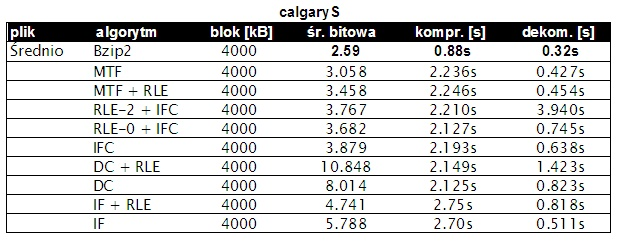
\includegraphics[scale=1.0]{\PICSDIR/tab_calgaryS_wszystkie.jpg}
\caption{\label{fig:tab_calgaryS_wszystkie.jpg}Wyniki testu dla zbioru calgaryS}
\end{figure}

\begin{figure}[phtb]
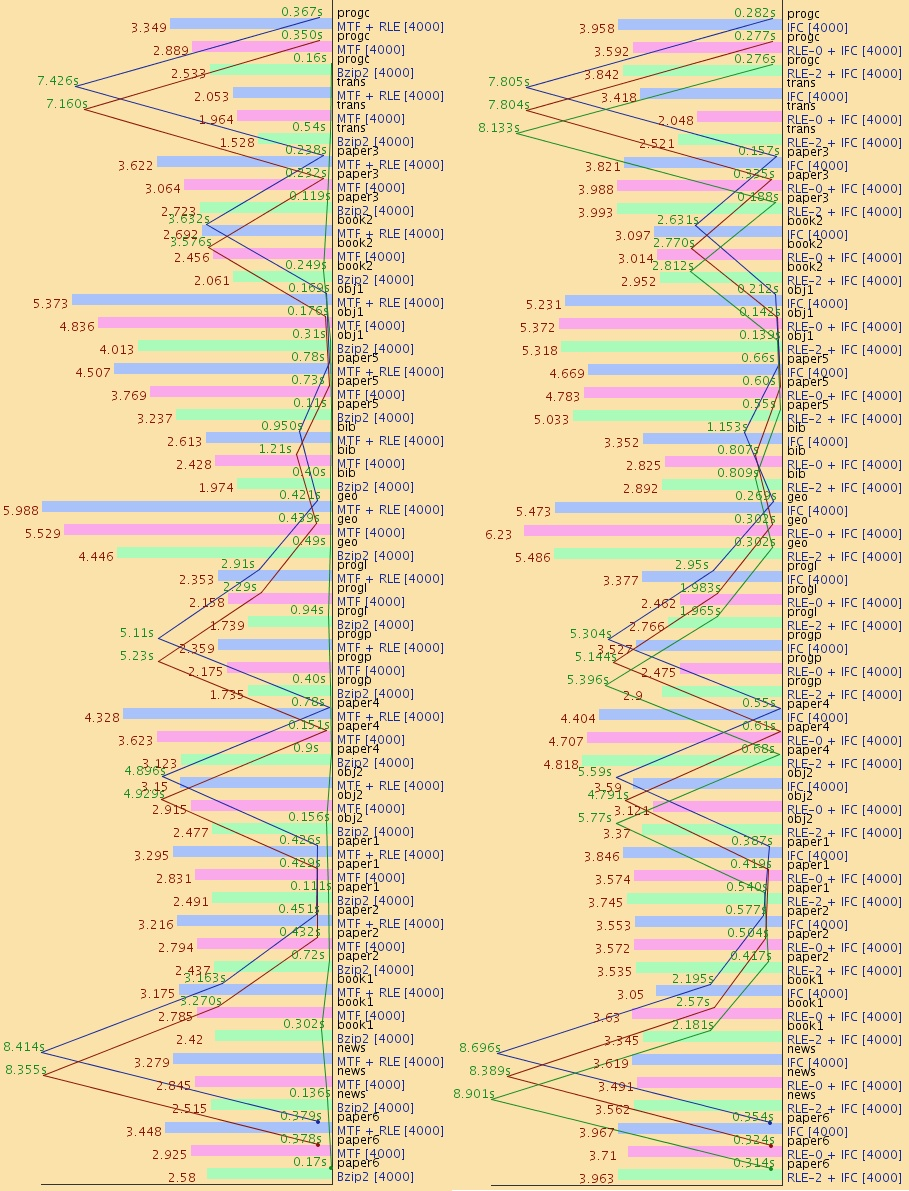
\includegraphics[scale=0.7]{\PICSDIR/graph_calgaryS_Bzip2_MTF_IFC.jpg}
\caption{\label{fig:graph_calgaryS_Bzip2_MTF_IFC.jpg}Wyniki testu dla zbioru calgaryS, algorytmy MTF i IFC}
\end{figure}

\begin{figure}[phtb]
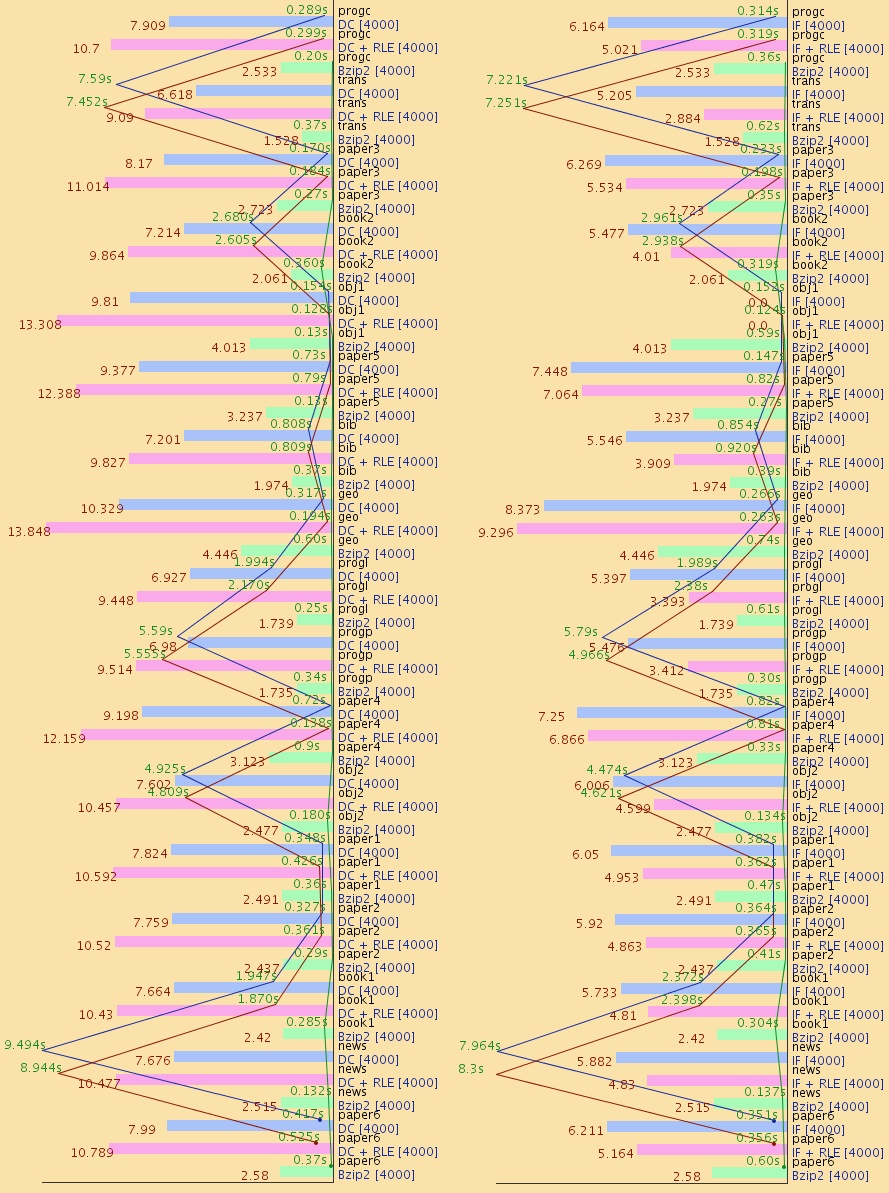
\includegraphics[scale=0.7]{\PICSDIR/graph_calgaryS_Bzip2_DC_IF.jpg}
\caption{\label{fig:graph_calgaryS_Bzip2_DC_IF.jpgg}Wyniki testu dla zbioru calgaryS, algorytmy DC i IF}
\end{figure}

\paragraph{Zbiór artificl}

Przeprowadzony został także test dla zbioru plików sztucznych. Algorytm MTF uzyskał najlepsze czasy kompresji dla pliku zawierającego pojedynczą literę ({\em a.txt}) oraz znaki w losowej kolejności ({\em random.txt}). Czasy te były lepsze także od czasów referencyjnego algorytmu Bzip2. Jednakże kompresja pozostałych dwóch plików zajęła kilka minut, a  średnie bitowe były gorsze.

\begin{figure}[phtb]
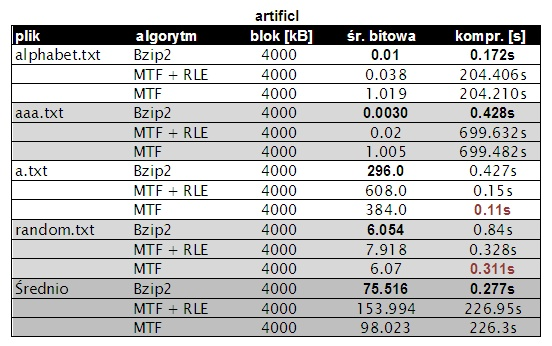
\includegraphics[scale=1.0]{\PICSDIR/tab_artificl_mtfrle.jpg}
\caption{\label{fig:tab_artificl_mtfrle.jpg}Wyniki testu dla zbioru artificl}
\end{figure}
